\documentclass[11pt]{article}
\usepackage{varnernotes}

\newcommand{\R}{\mathbb{R}}
\newcommand{\E}{\mathbb{E}}
\newcommand{\np}{|\mathcal P|}
\newcommand{\bw}{\mathbf w}
\newcommand{\bg}{\mathbf g}
\newcommand{\bn}{\mathbf n}
\newcommand{\bal}{\boldsymbol\alpha}
\newcommand{\bbe}{\boldsymbol\beta}
\newcommand{\Tan}{\mathcal T}
\newcommand{\Ap}{\mathcal A^{+}}
\newcommand{\Am}{\mathcal A^{-}}
\newcommand{\Rset}{\mathcal R}
\newcommand{\WP}{W_{\mathcal P}}
\newcommand{\Wadj}{W_{\mathrm{adj}}}
\newcommand{\SigSIM}{\hat\Sigma_{g,\mathrm{SIM}}}
\newcommand{\gSIM}{\hat{\bg}_{\mathrm{SIM}}}

\begin{document}

\lecturenotes{7a}{Utility-Based Allocation and the Adaptive Rebalancing Engine}{Fall 2026}{October 6, 2026}{Jeffrey D. Varner}

\learningobjectives
  {Explain why a static allocation fails}
  {Derive how buy-and-hold weights drift with prices and measure the drift, and state the three ways the minimum-variance inputs let the optimizer down: sensitivity to estimated means, concentration, and assumption fragility under regime change.}
  {Solve utility-based allocation problems}
  {Pose the budget-constrained maximum-utility problem, solve the Cobb--Douglas problem in closed form, state the CES solution and its three limits, and compute the preference weights from the SIM parameters and two market inputs, the recent market growth and a market-state signal.}
  {Build and score a rebalancing engine}
  {Write the self-financing account recursion with transaction costs and next-bar execution, state the reallocation schedule, turnover cap, and drawdown limit, and score a realized path by portfolio NPV, drawdown, realized growth and Sharpe ratio, turnover, and cost.}

\section{Allocation Is a Time-Stamped Decision}

L5b and L6b chose portfolio weights $\bw$ over $\np$ risky assets by solving a minimum-variance problem whose inputs were an expected growth-rate vector and a growth-rate covariance matrix; with the single index model of L6a those inputs are $\gSIM=\hat{\bal}+\hat{\bbe}\,g'_M$ and $\SigSIM=s^2_{g,M}\hat{\bbe}\hat{\bbe}^{\mathsf T}+\hat D_g$, where $\hat\alpha_i$ and $\hat\beta_i$ are the estimated intercept and beta of asset $i$, $g'_M$ and $s^2_{g,M}$ are the training-period sample mean and variance of the market growth rate, and $\hat D_g$ is the diagonal matrix of residual variances $s^2_{g,\varepsilon,i}$. For a target growth rate $g_\star$ the long-only weights $\bw(g_\star)$ minimize $\bw^{\mathsf T}\hat\Sigma_g\bw$ subject to $\bw^{\mathsf T}\hat{\bg}=g_\star$, $\mathbf 1^{\mathsf T}\bw=1$, $w_i\ge0$; the lowest point of the frontier is the global minimum-variance portfolio $\bw_{\mathrm{GMV}}$, and with a risk-free asset earning $g_f$ the fully invested point of the ray of risky/risk-free solutions is the tangent portfolio $\bw_{\Tan}$, the risky portfolio with the largest Sharpe ratio (quoted annualized, as in L6b).

Whatever the choice, it is implemented on a decision date $t=0$ by buying share counts $n_i=w_i\,\WP(0)/S_i(0)$, where $\WP(0)$ is the initial wealth and $S_i(0)$ the price of asset $i$; if nothing is traded afterward, the wealth on a later day is the share-weighted price aggregate:
\begin{equation}
  \label{eq:buy-and-hold}
  \WP(t)=\sum_{i\in\mathcal P}n_i\,S_i(t).
\end{equation}
The weights are optimal on the decision date, for the inputs estimated on that date. Nothing in the problem says they stay optimal, and the only decision the investor ever made was the one at $t=0$. These notes are about the other days.

\subsection*{Mechanical drift}

The weight of asset $i$ on day $t$ is its share of the portfolio's value, $w_i(t)=n_iS_i(t)/\WP(t)$. Substituting $n_i=w_i(0)\WP(0)/S_i(0)$ into numerator and denominator, the initial wealth cancels and the drifted weight depends only on the initial weights and the price relatives:
\begin{equation}
  \label{eq:drift}
  w_i(t)=\frac{w_i(0)\,\bigl(S_i(t)/S_i(0)\bigr)}{\sum_{j\in\mathcal P}w_j(0)\,\bigl(S_j(t)/S_j(0)\bigr)}.
\end{equation}

\begin{proposition}{When weights do not drift}{no-drift}
For every asset with $w_i(0)>0$, \eqnref{drift} gives $w_i(t)=w_i(0)$ if and only if every positively weighted asset has the same price relative $S_i(t)/S_i(0)$. Assets held at zero weight impose no condition. With the course convention $r_{i}=(\Delta t)g_{i}$ for the one-period log return ($\Delta t$ one trading day in years), the price relative over one period is $\exp((\Delta t)g_i)$ exactly; $1+(\Delta t)g_i$ is a small-move approximation.
\end{proposition}

We measure drift by the half-$L^1$ distance from the initial allocation:
\begin{equation}
  \label{eq:half-l1}
  \tfrac12\sum_{i\in\mathcal P}\lvert w_i(t)-w_i(0)\rvert,
\end{equation}
for a fully invested portfolio the fraction of wealth a rebalance back to the initial weights would have to trade on day $t$ before costs. Because $\sum_i w_i(t)=\sum_i w_i(0)=1$, the total weight lost by the assets that fell equals the total gained by those that rose, and the half counts each dollar that changes hands once. Drift also moves the modeled exposures: with fixed SIM betas the portfolio beta $\bw(t)^{\mathsf T}\hat{\bbe}$ changes with the weights, before any parameter is re-estimated (parameter drift is L7b's subject and is a second, separate source of change). In the drift example the SIM tangent portfolio held through 2025 ended the year with a drift of about $4.6\%$, NVDA's weight moved between $0.49$ and $0.58$, and the portfolio beta moved between $1.48$ and $1.54$.

\subsection*{Fragile inputs}

Drift is the benign failure. The optimizer's inputs are the serious one, and three tendencies of estimated minimum-variance and tangent portfolios recur. \emph{Input sensitivity}: the optimizer treats the estimated growth rates and covariances as exact, so estimation errors move the weights, and the tangent portfolio in particular overweights assets whose growth is overstated (Michaud's \emph{error maximizer}, 1989); Chopra and Ziemba (1993) showed that errors in the means matter far more than errors in the variances. \emph{Concentration}: without binding constraints the tangent portfolio, and often the GMV portfolio, puts most of its weight in a few names (the L6b tangent portfolio held four of thirteen firms). \emph{Assumption fragility}: the framework assumes one stable multivariate distribution, but correlations rise and volatilities jump in the episodes that matter. Two responses follow. Change the \emph{objective}, writing the investor's preferences for each asset down explicitly and letting them respond to the market state (these notes); or update the \emph{inputs} as data arrive (L7b).

\notebooklink
  {L7a: Drift of Maximum Sharpe Ratio Portfolios}
  {https://github.com/varnerlab/CHEME-5660-CourseRepository-Fall-2026/blob/main/lectures/week-7/L7a/CHEME-5660-L7a-Example-Portfolio-Drift-Fall-2026.ipynb}
  {Compute the tangent portfolio from SIM inputs, hold its share counts through 2025, and track the weights, the half-$L^1$ drift of \eqnref{half-l1}, and the portfolio's $\alpha$ and $\beta$.}

\section{From Preferences to an Allocation}

Instead of asking which portfolio has the smallest variance for a target growth rate, we ask a question from consumer choice theory: given a budget and today's market, which portfolio does the investor prefer most? A utility function assigns a real number to every feasible portfolio, larger for more preferred, and the investor maximizes it subject to the budget. At time $t$, with prices $S_i(t)$ (USD per share) and wealth $\WP(t)$ (USD), the general problem is
\begin{equation}
  \label{eq:utility-problem}
  \max_{n_1,\ldots,n_{\np}\ge0}\;U(n_1,\ldots,n_{\np})
  \qquad\text{subject to}\qquad
  \sum_{i\in\mathcal P}n_iS_i(t)=\WP(t).
\end{equation}
This is a \emph{holding} utility, a preference over the shares held today at today's prices; it is not the expected utility $\E[u(\WP(T))]$ of an uncertain terminal wealth $\WP(T)$ at a horizon $T$, and it is not risk-aware by itself. Risk enters through the preferences, which depend on the SIM betas and on the market state, and through the engine's rules. The proposal of this unit is that the preferences are computed each trading day, and that they answer two coupled questions: which assets belong in the basket today, and how much of each. The utility functions of the next section answer the second; the preference model of Section~4 answers the first.

\section{The Closed-Form Maximum-Utility Portfolio}

Let $\gamma_i\in(-1,1)$ be the preference weight of asset $i$. Its \emph{sign} classifies the assets into the preferred set $\Ap=\{i:\gamma_i>0\}$, the basket, and the non-preferred set $\Am=\{i:\gamma_i\le0\}$, held at a floor of $n_{\min}\ge0$ shares each (one hundredth of a share in the examples). Let $\Wadj=\WP(t)-n_{\min}\sum_{k\in\Am}S_k(t)>0$ be the budget left for the preferred set and $\Gamma=\sum_{j\in\Ap}\gamma_j$.

\begin{theorem}{Cobb--Douglas allocation}{cd-optimum}
The Cobb--Douglas utility over the preferred set is $U(\bn)=\prod_{i\in\Ap}n_i^{\gamma_i}$ with $n_i>0$ on $\Ap$ and $n_i=n_{\min}$ on $\Am$. For $\Wadj>0$, $S_i(t)>0$, at least one preferred asset, and fractional shares, its unique budget-constrained maximizer is
\begin{equation}
  \label{eq:cd-shares}
  n_i^\star=\frac{\gamma_i}{\Gamma}\cdot\frac{\Wadj}{S_i(t)}\quad(i\in\Ap),
  \qquad
  n_i^\star=n_{\min}\quad(i\in\Am),
\end{equation}
so the dollar weight of a preferred asset within the preferred budget is its normalized preference weight, $S_i(t)n_i^\star/\Wadj=\gamma_i/\Gamma$, independent of prices; as a fraction of total wealth it is $(\gamma_i/\Gamma)\,\Wadj/\WP(t)$. If the preferred set is empty the allocation is the floors plus cash.
\end{theorem}

\begin{derivation}
Maximizing $U$ over $\Ap$ is the same as maximizing $\ln U=\sum_{i\in\Ap}\gamma_i\ln n_i$. With multiplier $\lambda$ on the budget over the preferred set, the first-order condition for asset $i$ is $\gamma_i/n_i=\lambda S_i(t)$, i.e., $n_iS_i(t)=\gamma_i/\lambda$: each preferred asset receives dollars in proportion to its exponent. Summing over $\Ap$ gives $\Wadj=\Gamma/\lambda$, and substituting back gives \eqnref{cd-shares}. Strict concavity of $\ln U$ on the positive orthant (every $\gamma_i>0$ there) supplies uniqueness.
\end{derivation}

Sign classifies, magnitude allocates. The closed form applies to the preferred set only; a non-positive $\gamma_i$ is a classification, not an exponent to be inserted into \eqnref{cd-shares} (for $\gamma_i<0$ the term $n_i^{\gamma_i}$ grows without bound as $n_i\downarrow0$ and the theorem no longer applies), which is why the non-preferred assets are pinned at the floor. The allocation responds immediately to a change in $\gamma_i$: no covariance matrix, no quadratic program, no numerical solver.

\begin{proposition}{CES allocation and its limits}{ces}
For an elasticity of substitution $\eta>0$, $\eta\ne1$, the CES utility over the preferred set is $U_{\mathrm{CES}}(\bn)=\bigl(\sum_{i\in\Ap}\gamma_i n_i^{(\eta-1)/\eta}\bigr)^{\eta/(\eta-1)}$, and its budget-constrained maximizer is
\begin{equation}
  \label{eq:ces-shares}
  n_i^\star=\Wadj\;\frac{\bigl(\gamma_i/S_i(t)\bigr)^{\eta}}{\sum_{j\in\Ap}S_j(t)\bigl(\gamma_j/S_j(t)\bigr)^{\eta}}\quad(i\in\Ap).
\end{equation}
As $\eta\to1$ the allocation tends to the Cobb--Douglas allocation (the utility itself is undefined at $\eta=1$); as $\eta\to\infty$ the whole preferred budget goes to the asset with the largest $\gamma_i/S_i(t)$ (when unique); as $\eta\to0^+$ every preferred asset receives the same share count. The elasticity is a concentration dial. Because CES works with share counts, for $\eta\ne1$ its dollar weights $w_i^\star\propto S_i(t)^{1-\eta}\gamma_i^\eta$ depend on the price level of each share, which Cobb--Douglas weights do not.
\end{proposition}

The proofs are in the optional advanced notebook. The engine's CES variant ties the elasticity to the market-state signal $\xi_t$ of the next section (an EMA crossover on the market index, positive when the market has been falling), $\eta(\xi_t)=\eta_{\min}+(\eta_{\max}-\eta_{\min})/(1+\lvert\xi_t\rvert)$ with $0<\eta_{\min}\le\eta_{\max}$ ($0.5$ and $5$ in the examples): concentrate when the signal is quiet, diversify when it is loud in either direction. The log-linear utility $\sum_{i\in\Ap}\gamma_i\ln n_i$ is the logarithm of Cobb--Douglas: same maximizer, additive values.

\section{Preference Weights from the Single Index Model}

The preference weights come from the SIM parameters $(\alpha_i,\beta_i)$ of L6a and from two numbers that describe the market on day $t$: the recent market growth rate $\tilde g_{M,t}$, which plays the role of the SIM's expected market growth, and a scalar market-state signal $\xi_t$ (an EMA crossover on the market index, positive when the market has been falling; both are defined below):
\begin{equation}
  \label{eq:preference}
  \gamma_i(t)=\tanh\!\left(\frac{\alpha_i}{\beta_i^{\xi_t}}+\beta_i^{1-\xi_t}\,\tilde g_{M,t}\right).
\end{equation}
The hyperbolic tangent bounds the weight in $(-1,1)$. Its argument is the SIM's expected growth rate of asset $i$ in today's market, $\alpha_i+\beta_i\tilde g_{M,t}$ (units time$^{-1}$, read as a pure number at the one-year horizon), seen through a regime lens: since $\alpha_i/\beta_i^{\xi_t}+\beta_i^{1-\xi_t}\tilde g_{M,t}=(\alpha_i+\beta_i\tilde g_{M,t})/\beta_i^{\xi_t}$, the signal divides the expected growth by $\beta_i^{\xi_t}$.

\begin{proposition}{Sign classifies, magnitude allocates}{sign-magnitude}
Because $\beta_i^{\xi_t}>0$ and $\tanh$ preserves sign, $\operatorname{sign}\gamma_i(t)=\operatorname{sign}(\alpha_i+\beta_i\tilde g_{M,t})$: asset $i$ is preferred exactly when its expected growth in today's market is positive, $\tilde g_{M,t}>-\alpha_i/\beta_i$, and the signal $\xi_t$ never changes the classification. As the recent market growth moves, assets cross between the sets: a strong market pulls in firms with a small negative $\alpha_i$ and a large $\beta_i$, a weak market pushes out everything but the strongest intercepts, and when every $\gamma_i(t)\le0$ the model is saying that this basket does not belong in this market: the allocator holds the floors plus cash, and an investor not content with cash should rethink which assets are in the basket (the ticker-picking methods of L12b and L13a; the L7b update of $\alpha_i,\beta_i$ also moves the thresholds). The signal moves the magnitudes: a bearish $\xi_t>0$ divides by $\beta_i^{\xi_t}>1$ for high-beta names and by a number below one for low-beta names, tilting the preferred budget toward low-beta names, all else equal; a bullish $\xi_t<0$ tilts it toward high-beta names.
\end{proposition}

\begin{remark}{Assumptions behind the preference model}{preference-assumptions}
(i) $\beta_i>0$ for every asset, because $\beta_i$ is raised to a real power; the thirteen course firms have $\hat\beta_i$ between $0.54$ and $1.75$ and the examples assert it (a universe with a non-positive beta needs a rule for that asset, for example assignment to $\Am$). (ii) The argument is a growth rate in inverse years read as a pure number at the one-year horizon, which is why $\alpha_i$ and $\tilde g_{M,t}$ enter in annualized units. (iii) The recent market growth is a short exponential moving average of the daily market growth rates and swings by about a unit per year, an order of magnitude more than the intercepts: that is what makes the basket respond to the market, and it is why the engine's schedule and rules, not the model, decide how often the response is acted on.
\end{remark}

Both market inputs are computed from the market index (SPY) with exponential moving averages, $\bar S_t=\omega S_t+(1-\omega)\bar S_{t-1}$, $\omega=2/(L+1)$, for a window of $L$ trading days. With $L_{\mathrm{short}}=21$ and $L_{\mathrm{long}}=63$ and a dimensionless gain $G>0$, the market-state signal is the scaled crossover of the two price EMAs,
\begin{equation}
  \label{eq:signal}
  \xi_t=-G\left(\frac{\bar S^{\mathrm{short}}_t}{\bar S^{\mathrm{long}}_t}-1\right),
\end{equation}
positive (bearish) in a falling market and negative (bullish) in a rising one; $G$ is chosen on the training data so that $\lvert\xi_t\rvert\le1$ on 99\% of training days after a warm-up of $t_0=L_{\mathrm{short}}+L_{\mathrm{long}}$ days ($G\approx21$ on the course data). The recent market growth $\tilde g_{M,t}$ is the EMA with window $L_{\mathrm{growth}}=10$ of the daily market growth rates $g_{M,t}=\ln(S_t/S_{t-1})/\Delta t$ (time$^{-1}$). Both inputs on day $t$ are computed from prices through day $t-1$ (next section). On the last training day the signal was $-0.28$ and the recent market growth $-0.76$ per year, below every firm's threshold, so on the first trading day of 2025 no firm was preferred.

\notebooklink
  {L7a: Building a Maximum-Utility Portfolio Allocator}
  {https://github.com/varnerlab/CHEME-5660-CourseRepository-Fall-2026/blob/main/lectures/week-7/L7a/CHEME-5660-L7a-Example-Utility-Allocator-Fall-2026.ipynb}
  {Compute the market inputs and the preference weights \eqnref{preference} of thirteen firms on the first trading day of 2025 (basket empty) and on the first day the basket is nonempty (January 6: AAPL, MSFT, AMD, NVDA), the Cobb--Douglas allocation \eqnref{cd-shares} by hand and with the package (weights NVDA $0.59$, AMD $0.15$, AAPL $0.13$, MSFT $0.12$, floors eleven dollars of the thousand), the CES sweep of \eqnref{ces-shares} ($\eta=5$ puts 99\% in NVDA), and the comparison with the L6b GMV and tangent portfolios.}

\section{From Targets to Feasible Trades}

The allocator answers ``what would I hold right now?'' The engine asks it on a schedule and decides whether, and how much, to trade. Each bar is one pass through four stages, observe, orient, decide, act, shown in \figref{engine-loop}; a static allocation is one pass on the decision date followed by nothing.

\begin{figure}[ht]
  \centering
  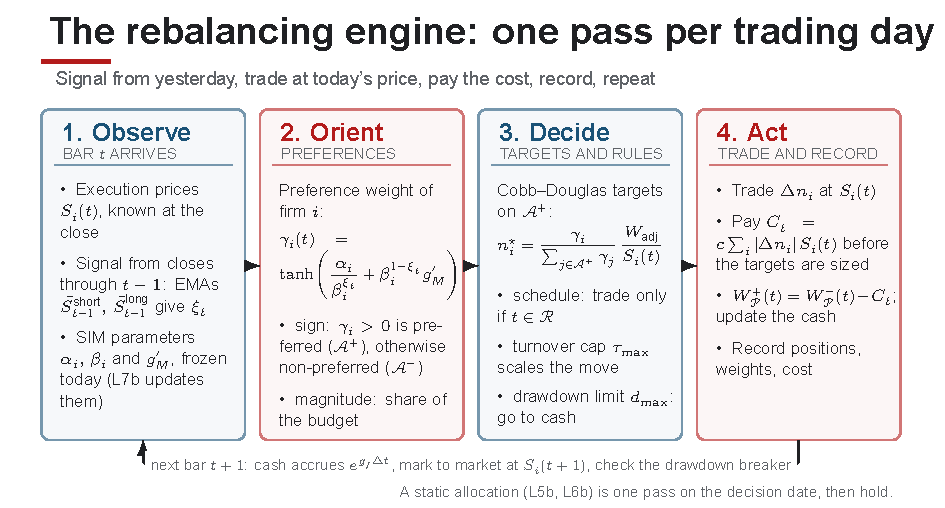
\includegraphics[width=\textwidth]{../figs/Fig-L7a-Rebalancing-Engine-Loop.pdf}
  \caption{The rebalancing engine as one pass per trading day: the market inputs come from closes through $t-1$, the preference weights and targets are computed, the rules are applied, and the trade executes at the close $S_i(t)$ with the cost taken out of the book as the trade is sized.}
  \label{fig:engine-loop}
\end{figure}

\subsection*{The self-financing account}

Let $n_{i,t}$ be the shares of asset $i$ held after the close of day $t$ and $\mathrm{cash}_t$ the cash after that close. Cash earns the risk-free growth rate, so during day $t$ it grows by $e^{g_f\Delta t}$, and at the close the book, before any trade, is worth
\begin{equation}
  \label{eq:mark}
  W^-_{\mathcal P}(t)=\mathrm{cash}_{t-1}\,e^{g_f\Delta t}+\sum_{i\in\mathcal P}n_{i,t-1}S_i(t),
\end{equation}
the superscript minus meaning ``before today's trades''. If the engine trades share deltas $\Delta n_i=n_{i,t}-n_{i,t-1}$ at the close prices $S_i(t)$, the gross notional traded is $Q_t=\sum_i\lvert\Delta n_i\rvert S_i(t)$ and, with $c$ the cost rate in dollars of cost per dollar traded ($5\times10^{-4}$ in the examples), the transaction cost is $C_t=c\,Q_t$. The cost comes out of the book and the new positions are sized against what is left,
\begin{equation}
  \label{eq:post-cost}
  W^+_{\mathcal P}(t)=W^-_{\mathcal P}(t)-C_t;
\end{equation}
because the cost depends on the trade and the trade on the post-cost budget, the engine solves the two together, iterating $C_t=c\sum_i\lvert w^{\mathrm{target}}_i\,(W^-_{\mathcal P}(t)-C_t)-n_{i,t-1}S_i(t)\rvert$ to its fixed point (a contraction for $c<0.05$, a few steps), so that $\mathrm{cash}_t+\sum_in_{i,t}S_i(t)=W^+_{\mathcal P}(t)$ holds exactly and cash never goes negative. Sizing against $W^-_{\mathcal P}(t)$ and debiting the cost afterward leaves the account short by $C_t$.

\subsection*{One-way turnover and the three rules}

Let $\Delta w_i$ be the change of asset $i$'s weight in the rebalance (as a fraction of $W^-_{\mathcal P}(t)$) and $\Delta w_{\mathrm{cash}}=-\sum_i\Delta w_i$ the cash leg. The one-way turnover
\begin{equation}
  \label{eq:turnover}
  \tau_t=\tfrac12\Bigl(\sum_i\lvert\Delta w_i\rvert+\lvert\Delta w_{\mathrm{cash}}\rvert\Bigr)
\end{equation}
is the fraction of wealth that changes hands one way; the cost applies to the gross notional $Q_t$, twice the one-way turnover times wealth when the cash leg does not move. Three rules bound the engine: a \emph{reallocation schedule}, the set of trading days $\Rset$ on which the engine may trade (daily, or every 21 days); a \emph{turnover cap} $\tau_{\max}$, which scales a proposed move down so that $\tau_t\le\tau_{\max}$; and a \emph{drawdown limit} $d_{\max}$, a circuit breaker checked every day before the schedule that liquidates the book to cash (bypassing the cap) when $1-W^-_{\mathcal P}(t)/\max_{s\le t}W^-_{\mathcal P}(s)>d_{\max}$, holds cash for $n_{\mathrm{lock}}$ more days, and rebases the peak on the first scheduled trade after that; checked once a day after the loss, and paying a cost on the liquidation, it does not cap the recorded drawdown at $d_{\max}$. The rules interact: moving all of the wealth from cash into risky assets is a one-way turnover of one, so with $\tau_{\max}=0.5$ the engine is only half invested until its next scheduled day, at the start and after every return from the floors or from a lock.

\begin{remark}{Fractional shares and richer costs}{feasibility}
The closed forms give fractional share counts; whole-share markets require rounding, and rounding each asset independently can violate the budget. Bid--ask spreads, market impact, minimum lots, and taxes are richer cost models than the proportional rate $c$; a turnover-penalized objective $\sum_{i\in\Ap}\gamma_i\ln n_i-\phi\sum_iS_i(t)\lvert n_i-n_{i,t-1}\rvert$ with reluctance $\phi\ge0$, or a no-trade band, are the standard ways to keep tiny theoretical improvements from being traded away. The engine of these notes uses the proportional cost and the cap; the L4a order-book material is where spread and impact live.
\end{remark}

\section{Information Timing and Backtesting Without Look-Ahead}

The market inputs and the preference weights that drive the decision on day $t$ are computed from prices through day $t-1$, and the trade executes at the close of day $t$ (a market-on-close order fills at the closing price, known when it fills). This is next-bar execution: nothing in the decision uses information that was not available before the bar it trades on. A closing-price signal traded at that same close is look-ahead, and it inflates every backtest it touches; the second example asserts the lag in code by perturbing one day's price and checking that the day's decision does not move.

\medskip\noindent\textbf{Algorithm (rebalancing engine, backtest).} The engine is allocator-agnostic: given the close prices $S_i(t)$ for $t=1,\ldots,N$ trading days, the initial wealth $\WP(0)$ in cash, the set $\Rset$, the rule parameters $(c,\tau_{\max},d_{\max},n_{\mathrm{lock}})$, and a target function $\bw^\star(t,\mathrm{state})$ that returns risky weights ($w_i^\star\ge0$, $\sum_iw_i^\star\le1$, the remainder cash) given the day and the current state (pre-trade wealth, weights, shares, cash, and a copy of the day's execution prices), for $t=1,\ldots,N$: (1) accrue the cash by $e^{g_f\Delta t}$, mark to market at $S_i(t)$ to get $W^-_{\mathcal P}(t)$, update the running peak; (2) if the drawdown exceeds $d_{\max}$ and the book holds risky positions, liquidate at $S_i(t)$, pay $c$ on the notional sold, lock for $n_{\mathrm{lock}}$ more days, and go to (5); (3) if $t\in\Rset$ and not locked, ask the target function for $\bw^\star$ (rebasing the peak if this is the first trade after a lock), form the proposed change of weights, and scale it to $\tau_{\max}$ if needed; (4) solve the cost and the positions together on the post-cost budget, execute $\Delta n_i$ at $S_i(t)$, pay $C_t=c\,Q_t$, update the cash; (5) record wealth, cash, positions, weights, turnover, cost, whether the engine traded or was locked, and the count of interventions. Our target functions compute $\gamma_i(t)$ from the market inputs through day $t-1$ and return the Cobb--Douglas (or CES) allocation at the day's closing prices as weights; the Cobb--Douglas weights do not depend on those prices, the CES weights do (through the bang for the buck), a same-close price dependence rather than a signal dependence. The static baselines (buy-and-hold GMV, tangent, equal weights, SPY) are the same loop with a constant target and $\Rset=\{1\}$, so they pay the same costs and follow the same accounting. Walk-forward discipline applies to the rule parameters as it did to everything else in this unit: choose them on training or validation data and freeze them for the test year.

\section{Scoring a Realized Path}

Did the portfolio beat what the same dollars would have earned at the risk-free growth rate? For one initial outflow, one terminal value, and a constant $g_f$ over the horizon $T=N\Delta t$ years, the portfolio NPV is
\begin{equation}
  \label{eq:npv}
  \mathrm{NPV}(g_f,T)=-\WP(0)+\WP(T)\,e^{-g_fT},
\end{equation}
positive when the run beat holding cash at $g_f$; the risk-free portfolio has NPV zero and is the zero every risky run is measured against. Alongside it: the realized growth rate $\ln\bigl(\WP(T)/\WP(0)\bigr)/T$; the maximum drawdown $\max_t\bigl(1-\WP(t)/\max_{s\le t}\WP(s)\bigr)$; the realized Sharpe ratio of the daily wealth growth in excess of $g_f$, annualized as in L6b (mean of the daily excess log growth over its standard deviation, times $\sqrt{1/\Delta t}$); and the implementation quantities the static portfolios do not have, total one-way turnover, total cost, and the number of interventions. A scorecard is one row per run and these columns.

Everything on the scorecard describes one realized path: 2025 happened once. It says what each policy did, not how likely that outcome was; a fail rate (how often the portfolio ends below the risk-free baseline), a lower quantile of terminal wealth, or the average of the worst outcomes need many paths, which is L7b.

\notebooklink
  {L7a: Running the Adaptive Rebalancing Engine Through 2025}
  {https://github.com/varnerlab/CHEME-5660-CourseRepository-Fall-2026/blob/main/lectures/week-7/L7a/CHEME-5660-L7a-Example-Adaptive-Rebalancing-Scorecard-Fall-2026.ipynb}
  {Build the lagged market inputs and preference weights for every 2025 day (the basket was empty on 57 of 250 days and full on 152), run the engine on monthly and daily schedules with the rules on and off and a CES variant, run the buy-and-hold GMV, tangent, equal-weight, and SPY portfolios through the same accounting, and read the scorecard: with $\Rset$ every 21 days, $\tau_{\max}=0.5$, $d_{\max}=0.10$, and $c=5$ basis points the Cobb--Douglas engine made 12 scheduled trades, held only the floors plus cash (risky exposure below 2\% of wealth) on 50 days, never fired the breaker, and ended at $1.53$ times initial wealth with a $9.0\%$ drawdown, against $1.28$ ($31\%$ drawdown) for the buy-and-hold tangent portfolio, $1.38$ for GMV, $1.59$ for equal weights, and $1.17$ for SPY.}

\section*{Optional Advanced Material}

\notebooklink
  {L7a Advanced: CES Limits, the Elasticity Rule, and Log-Linear Utility}
  {https://github.com/varnerlab/CHEME-5660-CourseRepository-Fall-2026/blob/main/lectures/week-7/L7a/advanced/adaptive_utility/CHEME-5660-L7a-Advanced-CES-Limits-Fall-2026.ipynb}
  {Derive the CES closed form \eqnref{ces-shares} and prove its three limits, read the two limits of $\eta(\xi_t)$, show that log-linear utility has the Cobb--Douglas optimizer, and see why the CES allocation over share counts depends on the price level of each share when $\eta\ne1$.}

\newpage
\thispagestyle{fancy}
\keytakeaways
  {In these notes, we derived how a static allocation drifts and why its inputs are fragile, replaced the minimum-variance objective with explicit preferences and the Cobb--Douglas and CES allocators, computed the preferences from the single index model and two market inputs so that they choose the basket and the weights within it, wrapped the allocator in a rebalancing engine with a self-financing account, next-bar execution, and three trigger rules, and scored a realized path.}
  {Utility makes preferences explicit and Cobb--Douglas turns them into weights in closed form}
  {The sign of a preference weight puts an asset in or out of the basket, its magnitude sets the asset's share of the preferred budget as the normalized preference weight, independent of prices, and the CES elasticity is a concentration dial with Cobb--Douglas as its unit-elasticity limit.}
  {The SIM plus two market inputs supplies the preferences, and the rules bound the response}
  {The recent market growth decides, asset by asset, whether the SIM's expected growth in today's market is positive and so which assets belong in the basket (an empty basket is the model saying to rethink the basket or hold cash), the crossover signal tilts the magnitudes between high-beta and low-beta names, and the schedule, turnover cap, and drawdown limit decide when, how far, and whether the engine acts, with the cost taken out of the book as the trade is sized.}
  {A realized-path scorecard is one draw}
  {Portfolio NPV against cash, drawdown, realized growth and Sharpe ratio, turnover, cost, and interventions say what a policy did on the year that happened; the distribution of what it could have done needs many simulated paths.}
  {Next, in L7b, we let the SIM parameters themselves update as data arrive, replay the engine with frozen and with updated parameters on the realized year and on an ensemble of simulated futures, and read the distributional scorecard those paths allow.}

\begin{readinglist}
  \item Richard O. Michaud, \href{https://doi.org/10.2469/faj.v45.n1.31}{``The Markowitz Optimization Enigma: Is `Optimized' Optimal?''} \emph{Financial Analysts Journal} 45(1), 31--42 (1989).
  \item Vijay K. Chopra and William T. Ziemba, \href{https://doi.org/10.3905/jpm.1993.409440}{``The Effect of Errors in Means, Variances, and Covariances on Optimal Portfolio Choice,''} \emph{Journal of Portfolio Management} 19(2), 6--11 (1993).
  \item Hal R. Varian, \emph{Microeconomic Analysis}, 3rd ed. (1992), chapters on utility maximization and the Cobb--Douglas and CES functional forms.
  \item Stephen Boyd et al., \href{https://web.stanford.edu/~boyd/papers/pdf/multi_period_trading.pdf}{``Multi-Period Trading via Convex Optimization,''} \emph{Foundations and Trends in Optimization} 3(1), 1--76 (2017).
\end{readinglist}

\vfill
{\sffamily\footnotesize\color{vnmuted}\textbf{Educational use and risk notice.} These notes are for instruction only and do not constitute investment advice. Utility scores, signals, and engine outputs are model-dependent and are not investment recommendations.}

\end{document}
